\documentclass[11pt,a4paper]{article}
\usepackage[utf8]{inputenc}
\usepackage[french]{babel}
\usepackage[T1]{fontenc}
\usepackage{mathtools}
\usepackage{tikz}
\usepackage{amsmath, amssymb, amsthm}            
\usepackage{amstext, amsfonts, a4}
\usepackage{hyperref}
\usepackage[ruled,vlined, french, onelanguage]{algorithm2e}
\usepackage[left=2cm,right=2cm,top=2cm,bottom=2cm]{geometry}
\usepackage{multicol}
\def\ccB{\mathscr{B}}
\newcommand\numberthis{\addtocounter{equation}{1}\tag{\theequation}}


\begin{document}
%\begin{center}
%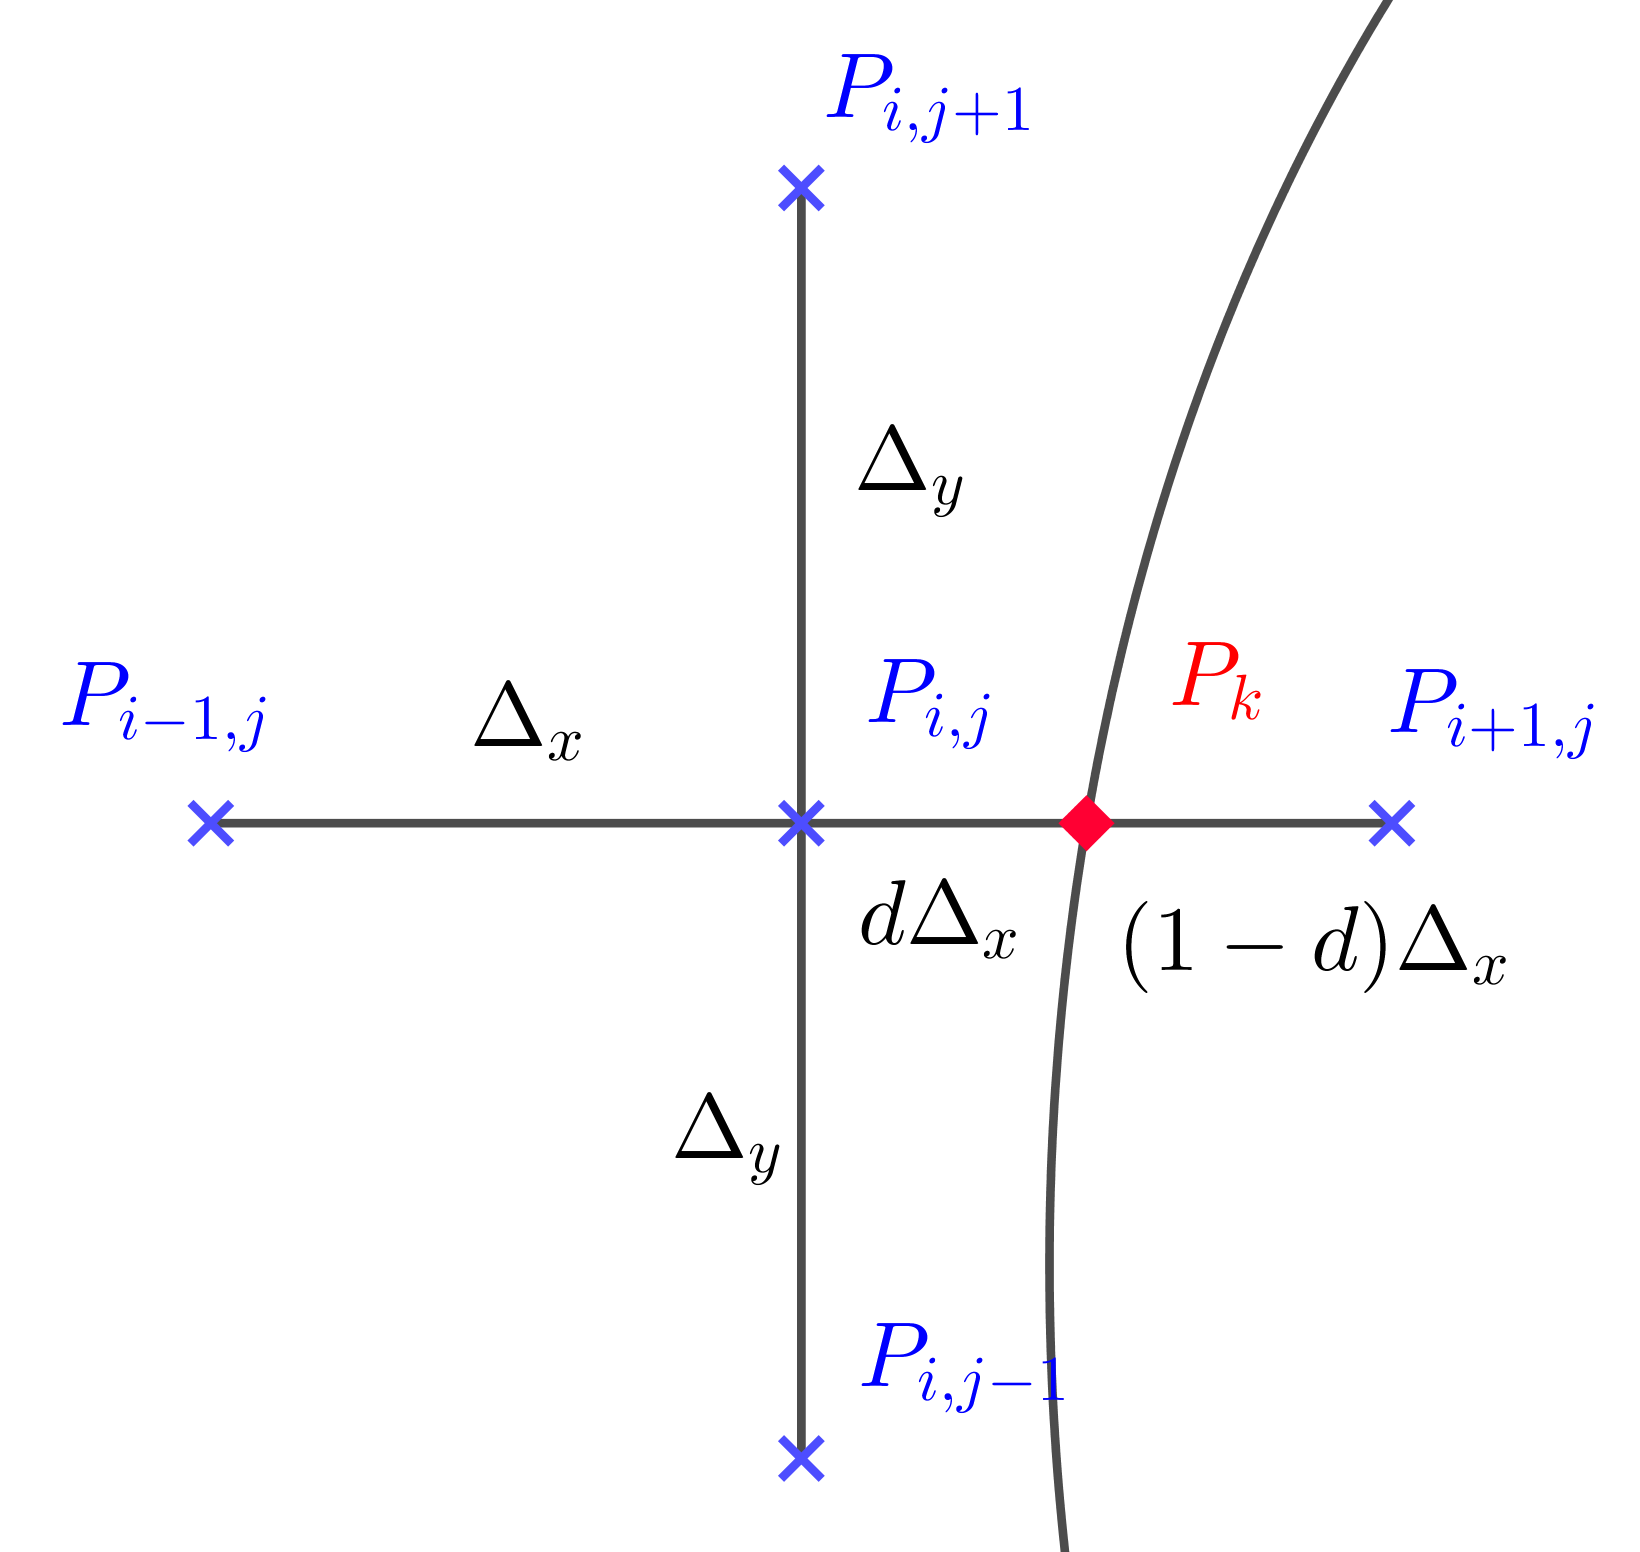
\includegraphics[scale=0.4]{graph_2d_mesh.png}
%\end{center}
Nous avons l'équation de la chaleur :
\begin{equation}
\partial_t\,u - D\,\Delta\,u = f\label{eq:heat}
\end{equation}
Discrétisée en 3D comme :
\begin{align*}
\frac{u^{n+1}_{i,j,k} - u^n_{i,j,k}}{\Delta t} &- D \left(\frac{u^{n+1}_{i-1,j,k} - 2\,u^{n+1}_{i,j,k}+u^{n+1}_{i+1,j,k}}{\Delta x^2} \right)\\
&-D \left(\frac{u^{n+1}_{i,j-1,k} - 2\,u^{n+1}_{i,j,k}+u^{n+1}_{i,j+1,k}}{\Delta y^2}\right)\\
&-D \left(\frac{u^{n+1}_{i,j,k-1} - 2\,u^{n+1}_{i,j,k}+u^{n+1}_{i,j,k+1}}{\Delta z^2}\right)= f_{i,j,k}^{n}
\end{align*}
Soient $a, b, c, d\in\mathbb{R}$ les coefficients d'interaction entre les points définis par
\begin{align*}
a := \frac{1}{\Delta t} -2b-2c-2d\hspace{1cm}b :=\frac{-D}{\Delta x^2}\hspace{1cm}c :=\frac{-D}{\Delta y^2}\hspace{1cm}d :=\frac{-D}{\Delta z^2}
\end{align*}
L'équation discrétisée devient donc
\begin{equation*}
a\,u_{i,j,k}^{n+1} + b\,\left(u_{i+1, j, k}^{n+1}+u_{i-1, j, k}^{n+1}\right) + c\,\left(u_{i, j+1, k}^{n+1}+u_{i, j-1, k}^{n+1}\right) + d\,\left(u_{i, j, k+1}^{n+1}+u_{i, j, k-1}^{n+1}\right) = \frac{1}{\Delta t}\,u_{i, j, k}^{n} + f_{i, j, k}^{n}
\end{equation*}
Étudions dans un premier temps $\eqref{eq:heat}$ avec conditions aux limites périodiques en 1D
\begin{equation*}
M_{1D}\left(\begin{array}{c}
u_{0, \cdot, \cdot}^{n+1}\\
\vdots\\
u_{N_x-1, \cdot, \cdot}^{n+1}
\end{array}\right) = \frac{1}{\Delta t} \left(\begin{array}{c}
u_{0, \cdot, \cdot}^{n}\\
\vdots\\
u_{N_x-1, \cdot, \cdot}^{n}
\end{array}\right) + \left(\begin{array}{c}
f_{0, \cdot, \cdot}\\
\vdots\\
f_{N_x-1, \cdot, \cdot}
\end{array}\right)
\end{equation*}
Avec
\begin{equation*}
M_{1D} = 
\begin{bmatrix}
a &b & & &b \\
b &\ddots &\ddots & & \\
 &\ddots &\ddots &\ddots &  \\
& &\ddots &\ddots  &b\\
b & & &b &a
\end{bmatrix}\in\mathcal{S}_{N_x}\left(\mathbb{R}\right)
\end{equation*}

Étudions dans un second temps $\eqref{eq:heat}$ avec conditions aux limites périodiques en 2D, extension vectoriel du cas 1D,
\begin{equation*}
M_{2D}\left(\begin{array}{c}
u_{0:N_x-1, 0, \cdot}^{n+1}\\
\vdots\\
u_{0:N_x-1, N_y-1, \cdot}^{n+1}
\end{array}\right) = \frac{1}{\Delta t} \left(\begin{array}{c}
u_{0:N_x-1, 0, \cdot}^{n}\\
\vdots\\
u_{0:N_x-1, N_y-1, \cdot}^{n}
\end{array}\right) +  \left(\begin{array}{c}
f_{0:N_x-1, 0, \cdot}^{n}\\
\vdots\\
f_{0:N_x-1, N_y-1, \cdot}^{n}
\end{array}\right)
\end{equation*}
Avec
\begin{equation*}
M_{2D} = 
\begin{bmatrix}
M_{1D} &C & & &C \\
C &\ddots &\ddots & & \\
 &\ddots &\ddots &\ddots &  \\
& &\ddots &\ddots  &C\\
C & & &C &M_{1D}
\end{bmatrix}\in\mathcal{S}_{N_xN_y}\left(\mathbb{R}\right)\text{ et }
C = 
\begin{bmatrix}
c & & \\
 &\ddots & \\
 & &c \\
\end{bmatrix}\in\mathcal{S}_{N_x}\left(\mathbb{R}\right)
\end{equation*}
Ainsi $\eqref{eq:heat}$ avec conditions aux limites périodiques en 3D, extension vectoriel du cas 2D,
\begin{equation*}
M_{3D}\left(\begin{array}{c}
u_{0:N_x-1, 0:N_y-1, 0}^{n+1}\\
\vdots\\
u_{0:N_x-1, 0:N_y-1, N_z-1}^{n+1}
\end{array}\right) = \frac{1}{\Delta t}\left(\begin{array}{c}
u_{0:N_x-1, 0:N_y-1, 0}^{n}\\
\vdots\\
u_{0:N_x-1, 0:N_y-1, N_z-1}^{n}
\end{array}\right) + \left(\begin{array}{c}
f_{0:N_x-1, 0:N_y-1, 0}^{n}\\
\vdots\\
f_{0:N_x-1, 0:N_y-1, N_z-1}^{n}
\end{array}\right)
\end{equation*}
Avec
\begin{equation*}
M_{3D} = 
\begin{bmatrix}
M_{2D} &D & & &D \\
D &\ddots &\ddots & & \\
 &\ddots &\ddots &\ddots &  \\
& &\ddots &\ddots  &D\\
D & & &D &M_{2D}
\end{bmatrix}\in\mathcal{S}_{N_xN_yN_z}\left(\mathbb{R}\right)\text{ et }
D = 
\begin{bmatrix}
d & & \\
 &\ddots & \\
 & &d \\
\end{bmatrix}\in\mathcal{S}_{N_xN_y}\left(\mathbb{R}\right)
\end{equation*}

Notre problème, regroupé sous forme matricielle sans conditions aux bords (sur la frontière définie par $\phi$) et en ajoutant les nouveaux points à la fin de ceux du maillage, devient :
\begin{equation*}
\underbrace{\left(
\begin{array}{c|c}
M_{3D} & 0\\
\hline
0 &\text{Id}
\end{array}\right)}_{:=A}\, U^{n+1} = \frac{1}{\Delta t}\,U^n + F
\end{equation*}

Il reste un problème à régler: les nouveaux points sont situés sur des arêtes du maillage. Il nous faut donc supprimer des anciennes interactions et en rajouter de nouvelles :
\begin{center}
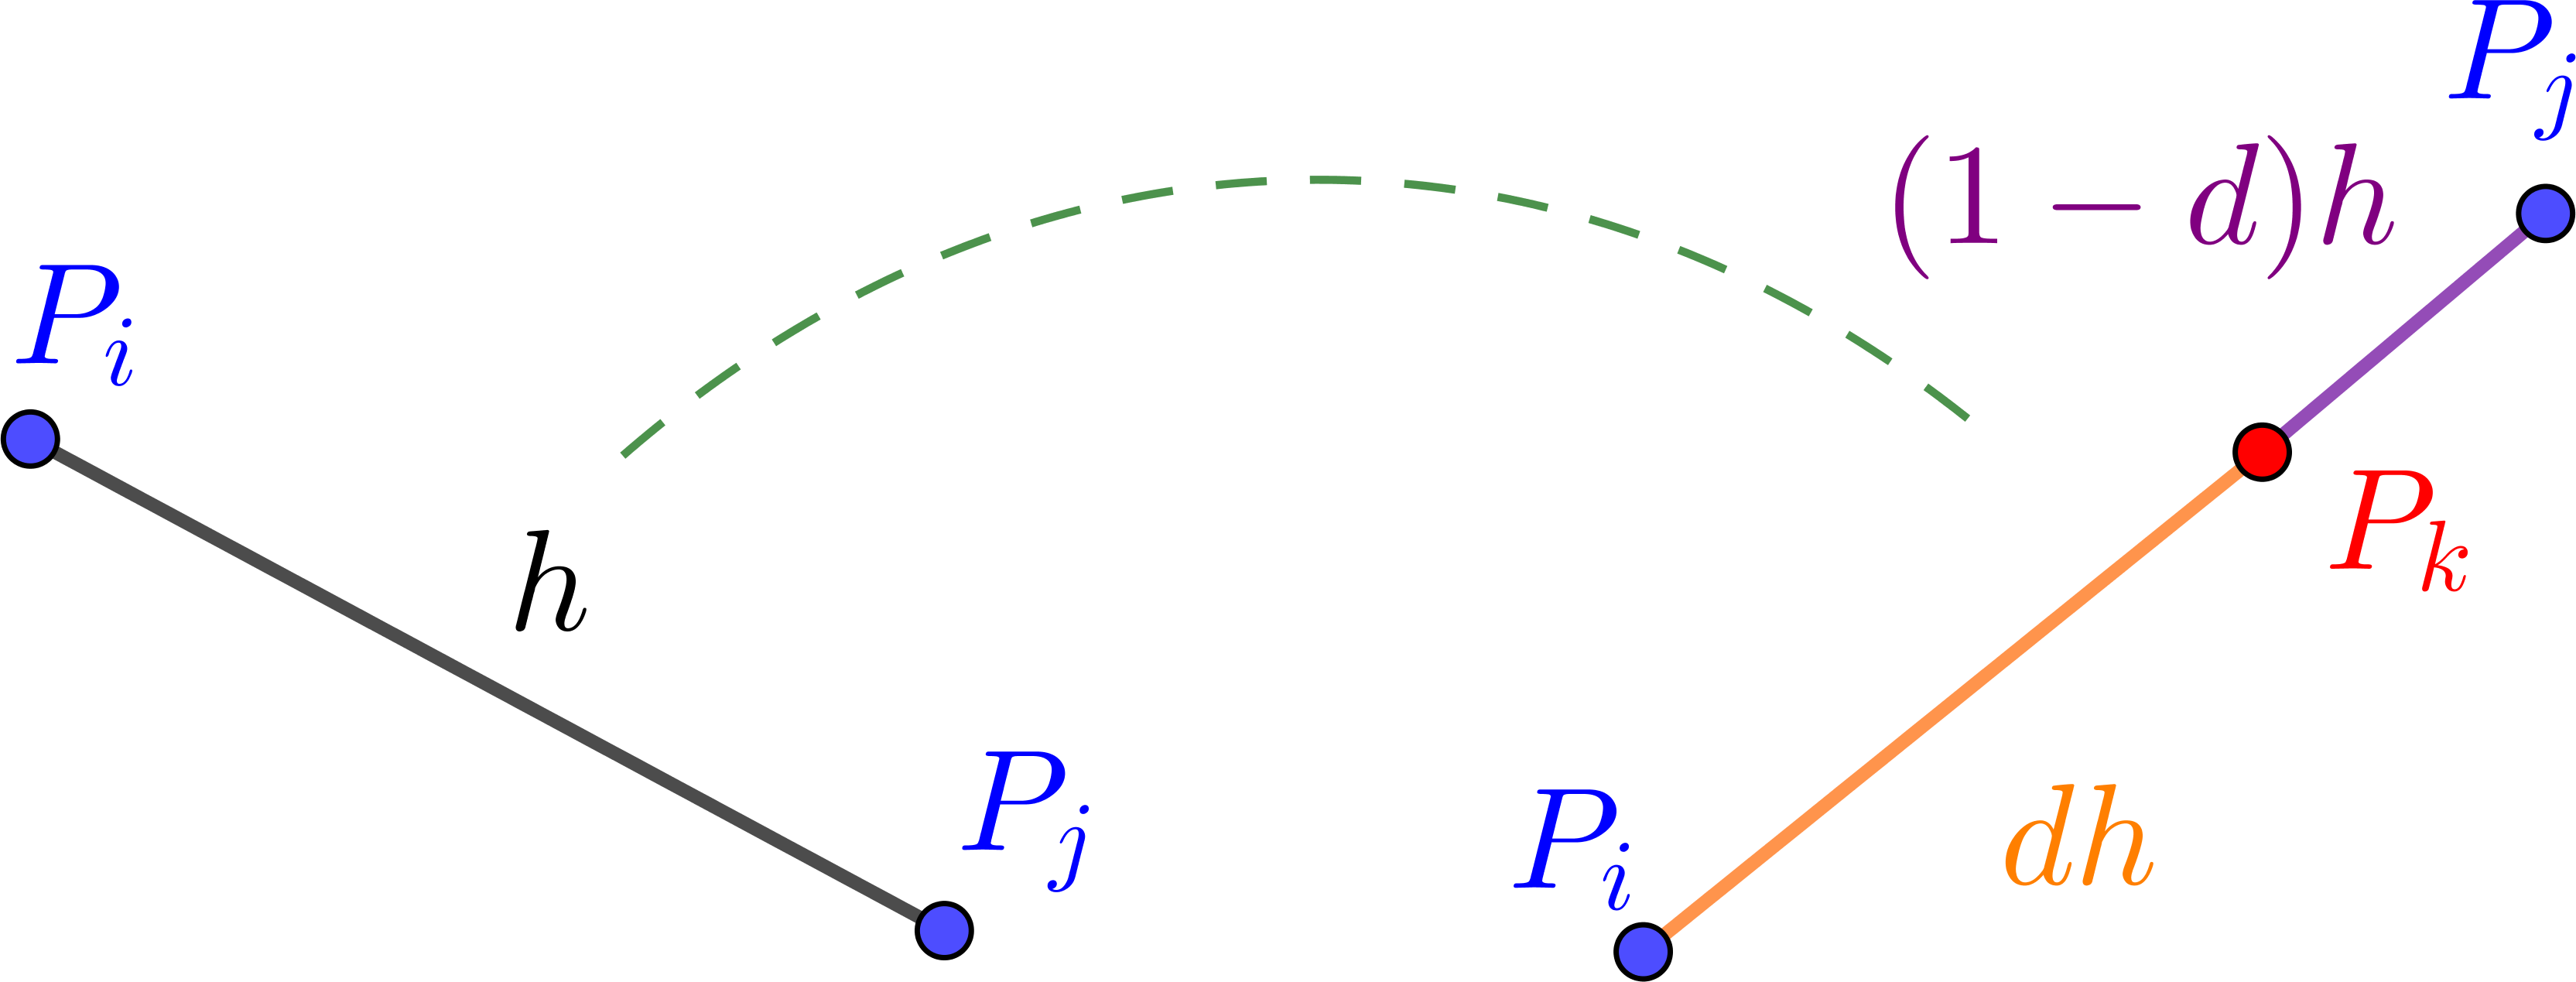
\includegraphics[scale=0.3]{changement.png}
\end{center}
Soient $P_i$ et $P_j$ deux points du maillage séparés par un pas $h$. Notons que sur un maillage cartésien $h$ peut uniquement être $\Delta x$, $\Delta y$ ou $\Delta z$.\\
Si nous insérons un point $P_k$ sur l'arête $[P_i, P_j]$ séparé de $P_i$ par une distance $hd$ et par une distance $(1-d)h$ de $P_j$, nous notons que $d\in[0,1]$ le facteur de changement de distance.\\

Si nous voulons découper l'ancienne interaction en deux nouvelles, il nous faut donc appliquer l'algorithme simpliste :
\begin{itemize}
\item \textbf{1)} Supprimer l'interaction entre $P_i$ et $P_j$. $A [i, j]= A [j, i] = 0$\\
\item \textbf{2)} Créer une interaction entre $P_i$ et $P_k$. Le coefficient est donné par $A [i, k] = A [k, i] = \frac{-D}{dh^2}$\\
\item \textbf{3)} Créer une interaction entre $P_j$ et $P_k$. Le coefficient est donné par $A [j, k] = A [k, j] = \frac{-D}{(1-d)h^2}$\\
\item \textbf{4)} Mettre à jour le coefficient diagonal pour le point $P_i$.\\
$A [i, i] = a + \frac{-D}{h^2} - \frac{-D}{dh^2} = \frac{1}{\Delta t} -2b -2c -2d + \frac{-D}{h^2} - \frac{-D}{dh^2}$\\
\item \textbf{5)} Mettre à jour le coefficient diagonal pour le point $P_j$.\\
$A [j, j] = a + \frac{-D}{h^2} - \frac{-D}{(1-d)h^2} = \frac{1}{\Delta t} -2b -2c -2d + \frac{-D}{h^2} - \frac{-D}{(1-d)h^2}$\\
\item \textbf{6)} Mettre à jour le coefficient diagonal pour le point $P_k$.\\
$A [k, k] = \frac{1}{\Delta t} - \frac{-D}{dh^2} - \frac{-D}{(1-d)h^2}$
\end{itemize}\vspace{15mm}
\textbf{Il en résulte une matrice à diagonale strictement dominante. Mais cela reste à prouver.}\vspace{10mm}\\
\newpage
L'algorithme un peu plus détaillé est celui-ci :\\
\begin{algorithm}[H]
\SetAlgoLined
\textbf{Définitions}\;
$\displaystyle b =\frac{-D}{\Delta x^2}, c=\frac{-D}{\Delta y^2}, d=\frac{-D}{\Delta z^2}, a = \frac{1}{\Delta t} -2b-2c-2d$\;
\ForEach{$p_k$ : point du bord}
{
	$k =$ indice global du point\;
	$n_k =$ nombre de voisins de $p_k$\;
	\If{$n_k = 2$}
	{
		\textbf{Le point $p_k$ est un point sur une arête}\;
		$p_i = $ premier voisin de $p_k$\;
		$i =$ indice global du point $p_i$\\
		$p_j = $ deuxième voisin de $p_k$\\
		$j =$ indice global du point $p_j$\\
		~\\
		$A [i,j] = A [j,i] = 0$ (supprime l'interaction entre $p_i$ et $p_j$)\\
		\textbf{Si }\textit{l'arête est sur l'axe $x$ }\textbf{Faire }\textit{Move ($\Delta x, b$)}\\
		\textbf{Si }\textit{l'arête est sur l'axe $y$ }\textbf{Faire }\textit{Move ($\Delta y, c$)}\\
		\textbf{Si }\textit{l'arête est sur l'axe $z$ }\textbf{Faire }\textit{Move ($\Delta z, d$)}\\
	}
	\If{$n_k = 4$}
	{
		\textbf{Le point est un point du maillage donc il n'y a rien de plus à faire}\\
	}
}
\caption{Idée}
\end{algorithm}

\begin{algorithm}[H]
\SetAlgoLined
$d = \frac{1}{h}\|p_k-p_i\|$\\
~\\
$v = \frac{1}{d} \times coeff$\\
$w = \frac{1}{(1-d)} \times coeff$\\
~\\
\textit{Màj de l'interaction entre $p_i$ et $p_k$}\\
$A [i, k] = A [k, i] = v$\\
$A [i, i] = A [i, i] + coeff - v$\\
~\\
\textit{Màj de l'interaction entre $p_j$ et $p_k$}\\
$A [j, k] = A [k, j] = w$\\
$A [j, j] = A [j, j] + coeff -  w$\\
~\\
\textit{Màj de la ligne $k$}\\
$A [k,k] = \frac{1}{\Delta t} - v - w$\\
\caption{Move (h, coeff)}
\end{algorithm}


\end{document}